\documentclass{article}
    \usepackage{amssymb}
    \usepackage{color}
    \usepackage{listings}
    \usepackage{graphicx}
    \usepackage{subcaption}
    \usepackage{geometry}
    \usepackage{float}
    \usepackage{caption}
    \usepackage{blindtext}
    \geometry{
    a4paper,
    total={170mm,257mm},
    left=20mm,
    top=20mm,
    }
    \DeclareCaptionFormat{citation}{%
    \ifx\captioncitation\relax\relax\else
      \captioncitation\par
    \fi
    #1#2#3\par}
 \newcommand*\setcaptioncitation[1]{\def\captioncitation{\textit{Source:}~#1}}
 \let\captioncitation\relax
 \captionsetup{format=citation,justification=centering}

    \setlength{\parindent}{0em}
    \setlength{\parskip}{1em} % length of the spacing
    
    \definecolor{gray}{rgb}{0.4,0.4,0.4}
    \definecolor{darkblue}{rgb}{0.0,0.0,0.6}
    \definecolor{cyan}{rgb}{0.0,0.6,0.6}
    
    \lstset{
      basicstyle=\ttfamily,
      columns=fullflexible,
      showstringspaces=false,
      commentstyle=\color{gray}\upshape
      frame=lr,
      framesep=8pt,
      framerule=0pt,
    }
    
    \lstdefinelanguage{XML}
    {
      morestring=[b]",
      morestring=[s]{>}{<},
      morecomment=[s]{<?}{?>},
      stringstyle=\color{black},
      identifierstyle=\color{darkblue},
      keywordstyle=\color{cyan},
      morekeywords={xmlns,version,type}% list your attributes here
      frame=lr,
      framesep=8pt,
      framerule=0pt,
    }
    \lstset{ % General setup for the package
        language=Python,
        basicstyle=\small\sffamily,
        numbers=left,
        numberstyle=\tiny,
        frame=tb,
        tabsize=4,
        columns=fixed,
        showstringspaces=false,
        showtabs=false,
        keepspaces,
        commentstyle=\color{red},
        keywordstyle=\color{blue},
        emphstyle=\ttb\color{deepred},    
        stringstyle=\color{blue}
    }

    
    \begin{document}

    \begin{titlepage}
        \begin{center}
            \vspace*{1cm}
            \begin{figure}
                \centering
                
\includegraphics[width=0.5\linewidth]{./img/vub.png}
            \end{figure}
            \Huge
            \textbf{Distributed Computing and Storage Architectures}
            
           
            
            \vspace{1.5cm}

            \textbf {\centering Juan Jose Soriano Escobar}
            \vspace{0.5cm}
            \newline
            \textbf{\centering Redona Brahimetaj}
            
            \vfill
            
            
            \Large
            Master in Applied Computer Science and Engineering\\
            Vrije Universiteit Brussels\\
            Brussels Belgium\\
            January 15, 2017
            
        \end{center}
    \end{titlepage}

    \tableofcontents
    \newpage

    \begin{appendix}
        \listoffigures
      \end{appendix}
      \newpage


        \section{Introduction}
        The importance of Distributed Computing is increasing a lot nowadays. It refers to a large collaboration between networked processing units that allows for their processing capacity to be put at the service of a large problem. Many systems and applications are being distributed for a variety of reasons: fault-tolerance, processing performance, security as well as geographical spreading of the data or the problem requirements. 
        
        In this project, we were asked to deploy an end-to-end big data harvesting and analysis chain which includes mining,processing and analysis of big data. The data that are being used, are taken from Twitter by using its public API to access them. These data, are tweets that represent million of opinions in many different topics. By deploying a Hadoop cluster and using MAP-REDUCE, we had to keep the most popular 10 hash-tags and words used as well as to count the number of occurrences of each word in the dataset. 
         
        \newpage         
        \section{Implementation Architecture}
        In this project, we tried to go further with the implementation by combining concepts that we learned in previous courses of the master, such as Web technologies and Databases.  
        We tried to simulate in a "real case" environment, where several devices with different applications or different back-end (e.g. mobile application in Python and web application in Nodejs) are used to collect a specific information and save it in a pre-defined database.

        \begin{figure}[H]
            \centering 
            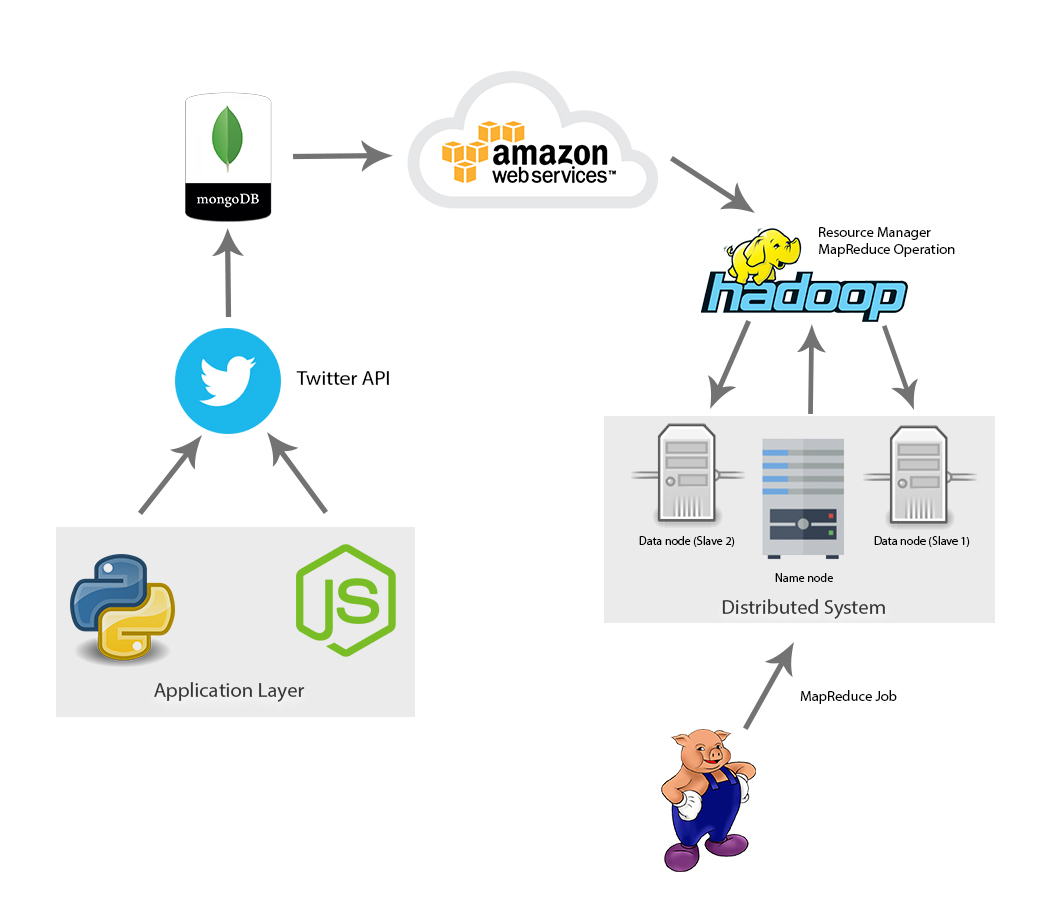
\includegraphics[width=1\linewidth]{./img/architecture.jpg}
            \setcaptioncitation{self-made}
            \caption{Distributed Computing Implementation.}
            \label{fig:architecture}
        \end{figure}

        In the Figure \ref{fig:architecture}, the global implementation that we used is Illustrated. At the bottom level, it presents how two different application in Python and Nodejs uses the Twitter API to recollect and save tweets in an MongoDB database. The idea behind this implementation is to illustrate how information could be retrieve from different sources and be processed as one data source.
        Consequently, the information is saved in a MongoDB database in an Amazon Web Server that is later connected with Hadoop distributed storage.

        At the same time, in Amazon Web server are three EC2 instances running with Hadoop with one NameNode as a master, assigning work to two slave nodes working as DataNodes to process the MapReduce task in parallel. Finally to create the MapReduce job, PIG framework (cite??) was implemented and installed in the name node as high-level platform which allows to use MapReduce tasks in a simple way, implementing a familiar SQL syntax.

        Finally the results are stored in the NameNode server and displayed in a simple HTML file.

        
        \section{Application layer}

        The application layer is related with the way how the data are retrieved and saved in the database by using Python and Javascript to access the Twitter API. In order to avoid the same implementation in two different programming languages,
        we decided to implement the solutions in two different scenarios. One implementing JavaScript without data processing and a second solution with Python  with the respective data cleaning and preprocessing, to
        visualize how the results of the top ten words and hashtags may change with a "clean" and "noisy" data. This comparison would show clearly the importance of having clean data and the impact it might have to the final results if the data is not preproccessed before.

        The code implemented for the Python implementation can be find in the github repository: % add description?

        The code implemented for the Nodejs implementation can be find in the github repository: % add description?

        \subsection{Data Pre-processing}

        The data preprocessing part is made by a function that receives the streamed tweet from the Twitter API and it tokenizes the tweet in words, to later remove the stop words, special characters, links, re-tweets and user tags. This step is required in order to extract the main words that potentially represent the meaning or topic of the tweet. Aditionally, Lemmatization is applied in the line \textit{13} to convert every word to the root 
        form, with the goal of grouping all the words that could semantically mean the same.
        \begin{lstlisting}[language=Python, caption= Python Cleaning Function, label={lst:dataCleaning}]
            def cleanTweet(tweet):    
                wordnet_lemmatizer = WordNetLemmatizer()
                stop = set(stopwords.words('english')) #stop words!
                framents = tknz.tokenize(tweet)
                clean_fragments = []
                for f in framents:
                    if f not in stop: # not included in the stop words
                        f = f.lower() #lowercase fragment
                        f = re.sub(r'[.,"!~_:|?\']+', '', f,flags=re.MULTILINE) # Special characters
                        f =  re.sub(r'\.\.\.', '', f,flags=re.MULTILINE)) # 3 dots
                        f = re.sub(url_expression, '', f,flags=re.MULTILINE) # links
                        f = re.sub(r'@[a-z,A-Z,0-9 ]*', '', f, flags=re.MULTILINE) #clean at person references
                        f = re.sub(r'RT @[a-z,A-Z]*: ', '', f, flags=re.MULTILINE) #Remove retweets
                        f = wordnet_lemmatizer.lemmatize(f)
                        if f:
                            clean_fragments.append(f)
                return(" ".join(clean_fragments))
        \end{lstlisting}

        \subsection{Twitter API Implementation}

        Implementation in Python....
        

        Implementation in Nodejs.....
        
        
        \section{Server Configuration}

        As  explained in section "look up" and presented in the Figure \ref{}, the server consist of one NameNode and two DataNodes running in different Linux instances in Amazon Web Services.

        Besides the security rules and after the Hadoop and Java installation, it was important to configure five files:
            \begin{itemize}
                \item \textbf{hadoop-env.sh:} This file contains some environment variable settings used by Hadoop. Frequenly use these to modify some aspects of Hadoop daemon behavior, such as where log files are stored, the maximum amount of heap used etc.                
                \item \textbf{core-site.xml:} contains the configuration of the name node and the temporal folder where the data is stored during the MapReduce process.
                \begin{lstlisting}[language=XML, caption= core-site.xml, label={lst:core}]
                    <?xml version="1.0" encoding="UTF-8"?>
                    <?xml-stylesheet type="text/xsl" href="configuration.xsl"?>
                    <configuration>
                    <property>
                      <name>fs.default.name</name>
                      <value>hdfs://namenode:8020</value>
                    </property>
                    <property>
                      <name>hadoop.tmp.dir</name>
                      <value>/home/ubuntu/hdfstmp</value>
                    </property>
                  </configuration>
                \end{lstlisting}
                \item \textbf{hdfs-site.xml:} contains the configuration for HDFS daemons, the NameNode, SecondaryNameNode  and data nodes.
                    \begin{lstlisting}[language=XML, caption= hdfs-site.xml, label={lst:hdfs}]
                        <?xml version="1.0" encoding="UTF-8"?>
                        <?xml-stylesheet type="text/xsl" href="configuration.xsl"?>
                        <configuration>
                        <property>
                          <name>dfs.replication</name>
                          <value>2</value>
                        </property>
                        <property>
                          <name>dfs.permissions</name>
                          <value>false</value>
                        </property>
                      </configuration>
                    \end{lstlisting}
                \item \textbf{mapred-site.xml:} contains the configuration settings for MapReduce daemons; it only need to specify in Hadoop that the yarn framework will be use for the map‐reduce jobs.
                    \begin{lstlisting}[language=XML, caption= mapred-site.xml, label={lst:mapred}]
                        <?xml version="1.0" encoding="UTF-8"?>
                        <?xml-stylesheet type="text/xsl" href="configuration.xsl"?>
                        <configuration>
                        <property>
                          <name>mapreduce.framework.name</name>
                          <value>yarn</value>
                        </property>
                      </configuration>                      
                \end{lstlisting}
                \item \textbf{yarn-site.xml:} the properties in this file specify where the ResourceManager is running so that other processes can connect to it.
                    \begin{lstlisting}[language=XML, caption= yarn-site.xml, label={lst:yarn}]
                        <?xml version="1.0" encoding="UTF-8"?>
                        <?xml-stylesheet type="text/xsl" href="configuration.xsl"?>
                        <configuration>
                        <!-- Site specific YARN configuration properties -->
                          <property>
                            <name>yarn.resourcemanager.resource-tracker.address</name>
                            <value>172.31.19.73:8031</value>
                          </property>
                          <property>
                            <name>yarn.resourcemanager.address</name>
                            <value>172.31.19.73:8032</value>
                          </property>
                          <property>
                            <name>yarn.resourcemanager.scheduler.address</name>
                            <value>172.31.19.73:8030</value>
                          </property>
                          <property>
                            <name>yarn.resourcemanager.admin.address</name>
                            <value>172.31.19.73:8033</value>
                          </property>
                          <property>
                            <name>yarn.resourcemanager.webapp.address</name>
                            <value>172.31.19.73:8088</value>
                          </property>
                          <property>
                            <name>yarn.nodemanager.aux‐services</name>
                            <value>mapreduce_shuffle</value>
                          </property>
                        </configuration>                     
                \end{lstlisting}
            \end{itemize}
        All the configuration files could be find in the github repository .....
        \begin{figure}[H]
            \centering 
            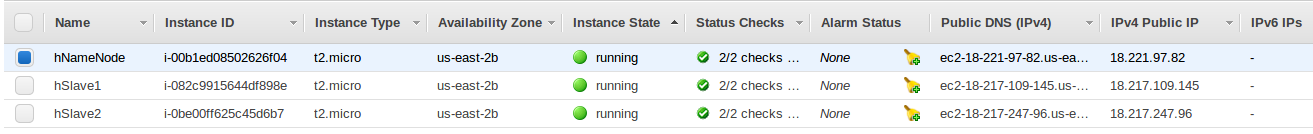
\includegraphics[width=1\linewidth]{./img/instances.png}
            \setcaptioncitation{Screenshot idk.}
            \caption{AWS instances.}
            \label{fig:instances}
        \end{figure}

        \section{MapReduce Job}

MapReduce is a framework that is used to process large amount of data in a distributed fashion over several machines. The core idea that stands behind MapReduce is mapping the data into a collection of <key,value> pairs and then reducing over all pairs with the same key. If we would have to explain it in more detailed steps, we would say that in the beggining the framework will split the data into segments passing each segment to a differen machine. Each machine then runs the map script on the portion of the data attributed to it. As it is already mentioned above, the map script takes the input data and maps it to <key,value> pairs according to the specifications that we give. In our case, the map script consisted of <word,count> to be our <key,value> pairs. Here it is very important to mention that we do not have aggregation since this is the task of the reduce script. The emitted <key,value> pairs are then shuffled which means that pairs with the same key are grouped and passed to a single machine which will then run the reduce script over them. The reduce script will take the <key,values> pairs and 'reduce' them according to the specified reduce script. In our word count example, we want to count the number of word occurrencies so on our reduce script we simply sum the values of the collection <key;value> pairs which have the same key. This is shown in figure \ref{fig:MapReduce}. 

\begin{figure}[H]
            \centering 
            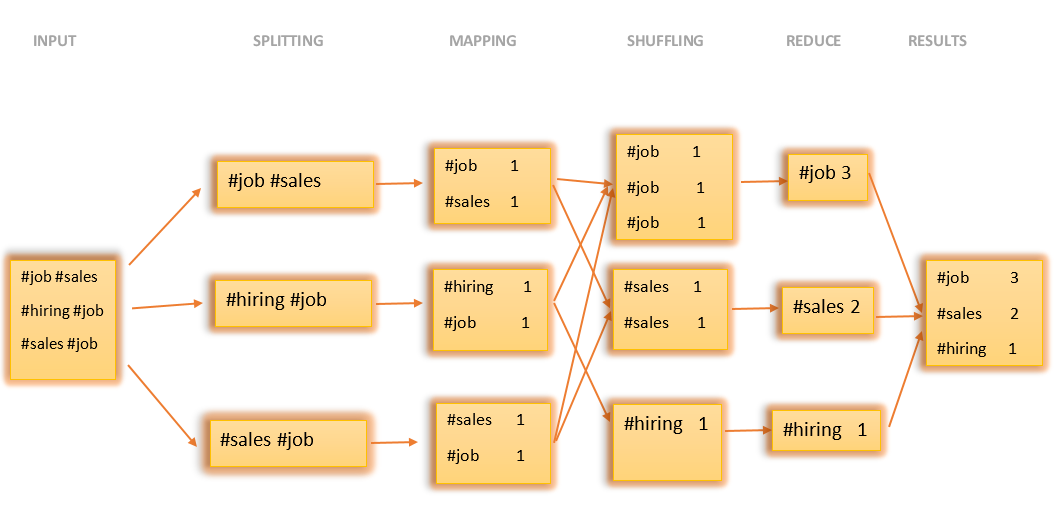
\includegraphics[width=1\linewidth]{./img/MapReduce.png}
            \setcaptioncitation{self-made}
            \caption{MapReduce process.}
            \label{fig:MapReduce}
        \end{figure}

        To build the MapReduce Job, Apache Pig was used to take advantage of it easy SQL oriented approach to program, increasing the productivity and friendly for programmers that have not use Java before.
        Ten line of code in Pig Latin are equivalent almost to 200 lines of code in Java. (http://blog.cloudera.com/wp-content/uploads/2010/01/IntroToPig.pdf)

        Apache Pig is then installed in the name node and connected to YARN to manage the job request. 
        
        In the listing \ref{} is provided the job use to calculate the top ten used words and the top ten hashtags. From a global overview, the COUNT in Apache Pig is equivalent to a reduce and the Filter is translated to a map.
        Additionally the tokenize also represent a  map function that split a string of words into a bag of words.

        \begin{lstlisting}[caption= Tweet cleaning function, label={lst:dataCleaning}]
            REGISTER /home/ubuntu/hadoop/share/hadoop/common/lib/mongo-java-driver-3.6.0.jar;
            REGISTER /home/ubuntu/hadoop/share/hadoop/common/lib/mongo-hadoop-pig-2.0.2.jar;
            REGISTER /home/ubuntu/hadoop/share/hadoop/common/lib/mongo-hadoop-core-2.0.2.jar;
            
            data = LOAD '/home/ubuntu/distributedComputing/tweets.bson'
                USING
                com.mongodb.hadoop.pig.BSONLoader('fullResponse','text') AS (text:chararray);
            
            words = FOREACH data  GENERATE FLATTEN(TOKENIZE(text)) as word;
            grouped = GROUP words BY word;
            wordcount = FOREACH grouped GENERATE group, COUNT(words);
            
            ordered = ORDER wordcount by $1 DESC;
            top_words = LIMIT ordered 10;
            hash_filter = FILTER ordered BY $0 MATCHES '.*\\#\\p{Alpha}.*?';
            
            top_hash = LIMIT hash_filter 10;

            STORE top_hash INTO '/home/ubuntu/pig/scripts/top_10_hash';
            STORE top_words INTO '/home/ubuntu/pig/scripts/top_10_words'

        \end{lstlisting}

        The first three register statements in the Pig Script is implementing the Java, MongoDB and Hadoop conectors to work across the the architecture defined for the 3 instances. Then
        the BSON file from the database is loaded and the tweet is saved as "text". In the following lines, the tokenize divides the tweets into words (map) to consequently group them.
        From that point it is needed to count the amount of times that a word is present in the all the tweets, using COUNT (filter).
        
        With the pair word and number of repetitions of the word, is just matter of order them in descended order to identify the top ten words and filter (reduce) all the words that start by the character \# to 
        extract also the top ten hashtags.

        Finally with the STORE command, the results are locally saved in the server.

        ** Apache Pig is a platform for analyzing large data sets that consists of a high-level language for expressing data analysis programs, coupled with infrastructure for evaluating these programs. 
        The salient property of Pig programs is that their structure is amenable to substantial parallelization, which in turns enables them to handle very large data sets. 
        (https://pig.apache.org/)

        ** YARN is the architectural center of Hadoop that allows multiple data processing engines such as interactive SQL, real-time streaming, data science and batch processing to handle data stored 
        in a single platform, unlocking an entirely new approach to analytics.
        https://hortonworks.com/apache/yarn/
        \section{Job Results}
		\pagebreak  
		\begin{figure}[H]
            \centering 
            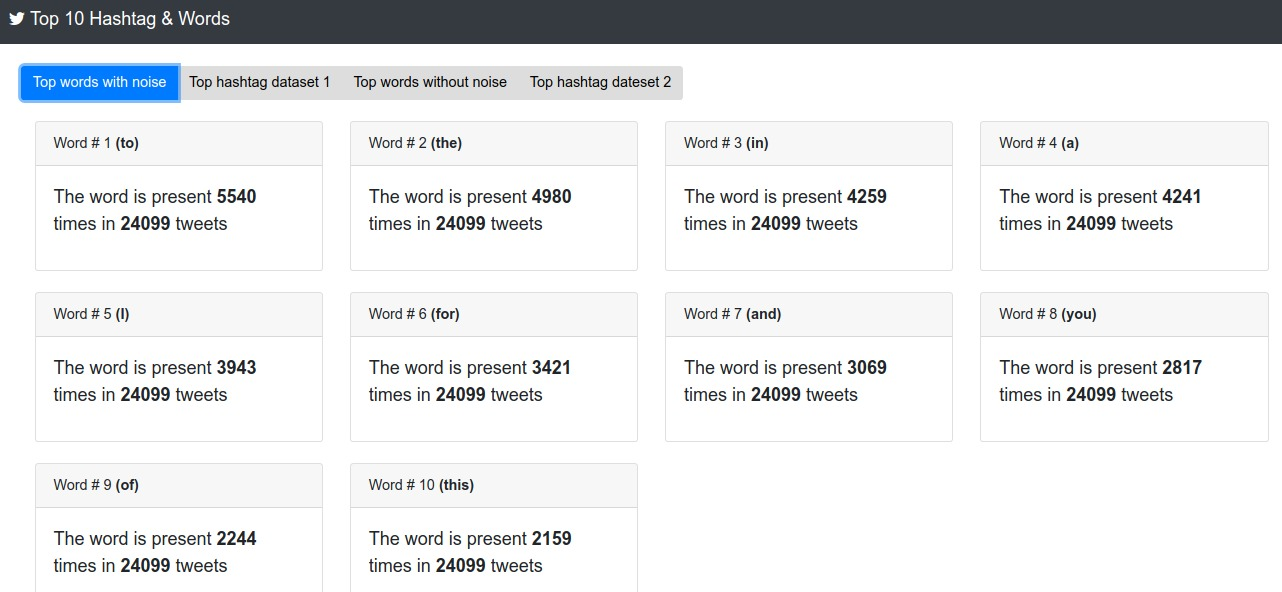
\includegraphics[width=1\linewidth]{./img/topwordswithnoise.jpeg}
            \setcaptioncitation{self-made}
            \caption{Top Words with Noise}
            \label{fig: Top Words with Noise}
        \end{figure}
        
        \begin{figure}[H]
            \centering 
            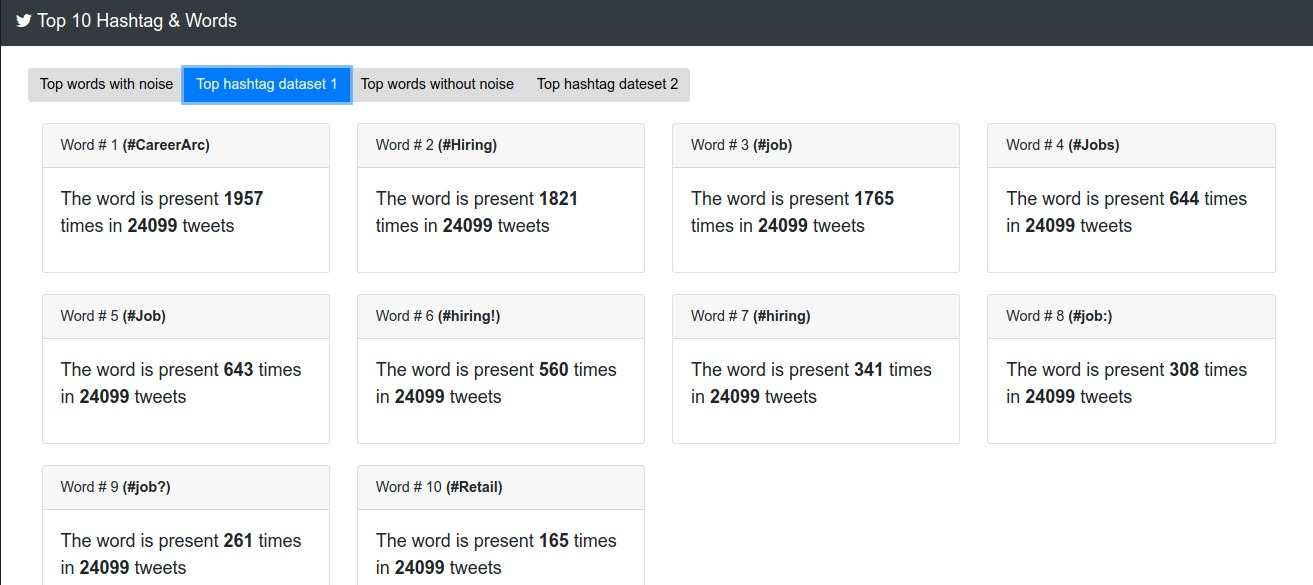
\includegraphics[width=1\linewidth]{./img/tophashtagdataset1.jpeg}
            \setcaptioncitation{self-made}
            \caption{Top Hashtag Dataset 1}
            \label{fig: Top Hashtag Dataset 1}
        \end{figure}
        
        \begin{figure}[H]
            \centering 
            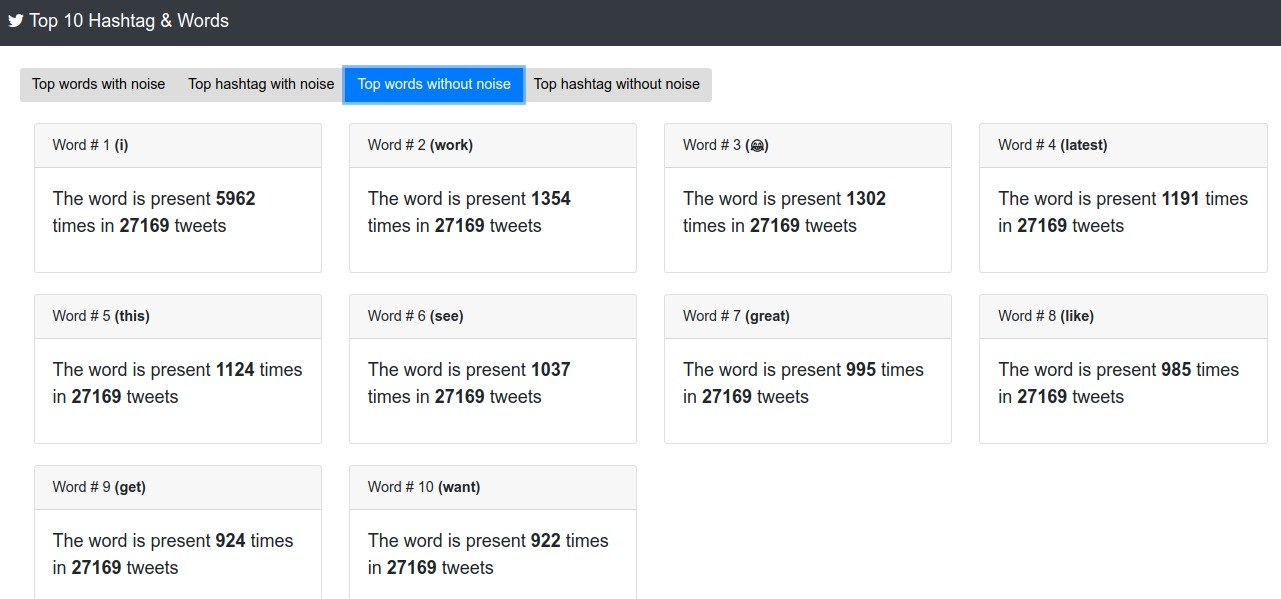
\includegraphics[width=1\linewidth]{./img/topwordswithoutnoise.jpeg}
            \setcaptioncitation{self-made}
            \caption{Top Words without Noise}
            \label{fig: Top Words without Noise}
        \end{figure}
        
        \begin{figure}[H]
            \centering 
            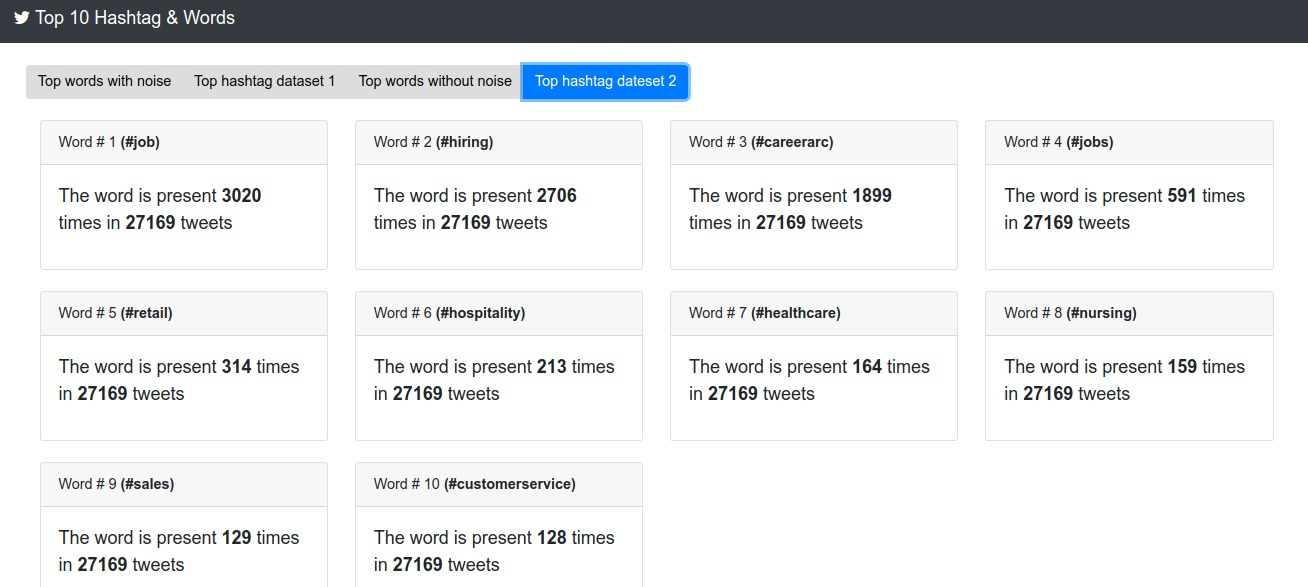
\includegraphics[width=1\linewidth]{./img/tophashtagdataset2.jpeg}
            \setcaptioncitation{self-made}
            \caption{Top Hashtag Dataset 2}
            \label{fig: Top Hashtag Dataset 2}
        \end{figure}
		      
        \section{Conclusion}
In this project, by using Twitter API we managed to have access to a large amount of tweets (27169 tweets retrieved using Python and 24099 tweets retrieved using Javascript). A very important step was the data cleaning since it leads to different results if the process is not done correctly. As it was also described in the project requirements, we splitted the raw data into meaningful components by taking only the root of the words, removing punctuation marks ecc.

 As a storage, we used MongoDB since we stored all the data there.This information is saved in an Amazon Web Server that is later connected with Hadoop distibuted Storage. Hadoop has become a key tool for managing pools of big data and supporting big data analytics applications.It takes the data,breaks the information down into separate pieces and distributes them to different nodes in a cluster, in our case in 2 slave nodes, allowing for parallel processing. The file system also copies each piece of data multiple times and distributes the copies to individual nodes, placing at least one copy on a different server rack than the others. The best advantage that we profit from using it, is the time. We processed more than 20000 tweets in less than 5 seconds

To express more clearly the difference between having cleaned and uncleaned data, we decided to present two types of scenarios, one where we used JavaScript to retrieve the data and we did not preprocess them, and one where we used Python to retrieve and preprocess. The differences are shown clearly. When the data is unprocessed and we apply MAP-REDUCE, the result we get when we want to find the top 10 most used words and the number of times they are found, influences the effectiveness of the whole process since we get as a result stop words that does not express the core idea of the task. Meanwhile, when the data was preprocessed, the words that we got as a result were meaningful and they expressed exactly the most used words among all the tweet.


      
    \bibliography{report}
    \bibliographystyle{ieeetr}
    \nocite{*}
\end{document}